% Options for packages loaded elsewhere
\PassOptionsToPackage{unicode}{hyperref}
\PassOptionsToPackage{hyphens}{url}
\PassOptionsToPackage{dvipsnames,svgnames,x11names}{xcolor}
%
\documentclass[
  authoryear,
  preprint,
  3p]{elsarticle}

\usepackage{amsmath,amssymb}
\usepackage{iftex}
\ifPDFTeX
  \usepackage[T1]{fontenc}
  \usepackage[utf8]{inputenc}
  \usepackage{textcomp} % provide euro and other symbols
\else % if luatex or xetex
  \usepackage{unicode-math}
  \defaultfontfeatures{Scale=MatchLowercase}
  \defaultfontfeatures[\rmfamily]{Ligatures=TeX,Scale=1}
\fi
\usepackage{lmodern}
\ifPDFTeX\else  
    % xetex/luatex font selection
\fi
% Use upquote if available, for straight quotes in verbatim environments
\IfFileExists{upquote.sty}{\usepackage{upquote}}{}
\IfFileExists{microtype.sty}{% use microtype if available
  \usepackage[]{microtype}
  \UseMicrotypeSet[protrusion]{basicmath} % disable protrusion for tt fonts
}{}
\makeatletter
\@ifundefined{KOMAClassName}{% if non-KOMA class
  \IfFileExists{parskip.sty}{%
    \usepackage{parskip}
  }{% else
    \setlength{\parindent}{0pt}
    \setlength{\parskip}{6pt plus 2pt minus 1pt}}
}{% if KOMA class
  \KOMAoptions{parskip=half}}
\makeatother
\usepackage{xcolor}
\setlength{\emergencystretch}{3em} % prevent overfull lines
\setcounter{secnumdepth}{5}
% Make \paragraph and \subparagraph free-standing
\ifx\paragraph\undefined\else
  \let\oldparagraph\paragraph
  \renewcommand{\paragraph}[1]{\oldparagraph{#1}\mbox{}}
\fi
\ifx\subparagraph\undefined\else
  \let\oldsubparagraph\subparagraph
  \renewcommand{\subparagraph}[1]{\oldsubparagraph{#1}\mbox{}}
\fi

\usepackage{color}
\usepackage{fancyvrb}
\newcommand{\VerbBar}{|}
\newcommand{\VERB}{\Verb[commandchars=\\\{\}]}
\DefineVerbatimEnvironment{Highlighting}{Verbatim}{commandchars=\\\{\}}
% Add ',fontsize=\small' for more characters per line
\usepackage{framed}
\definecolor{shadecolor}{RGB}{241,243,245}
\newenvironment{Shaded}{\begin{snugshade}}{\end{snugshade}}
\newcommand{\AlertTok}[1]{\textcolor[rgb]{0.68,0.00,0.00}{#1}}
\newcommand{\AnnotationTok}[1]{\textcolor[rgb]{0.37,0.37,0.37}{#1}}
\newcommand{\AttributeTok}[1]{\textcolor[rgb]{0.40,0.45,0.13}{#1}}
\newcommand{\BaseNTok}[1]{\textcolor[rgb]{0.68,0.00,0.00}{#1}}
\newcommand{\BuiltInTok}[1]{\textcolor[rgb]{0.00,0.23,0.31}{#1}}
\newcommand{\CharTok}[1]{\textcolor[rgb]{0.13,0.47,0.30}{#1}}
\newcommand{\CommentTok}[1]{\textcolor[rgb]{0.37,0.37,0.37}{#1}}
\newcommand{\CommentVarTok}[1]{\textcolor[rgb]{0.37,0.37,0.37}{\textit{#1}}}
\newcommand{\ConstantTok}[1]{\textcolor[rgb]{0.56,0.35,0.01}{#1}}
\newcommand{\ControlFlowTok}[1]{\textcolor[rgb]{0.00,0.23,0.31}{#1}}
\newcommand{\DataTypeTok}[1]{\textcolor[rgb]{0.68,0.00,0.00}{#1}}
\newcommand{\DecValTok}[1]{\textcolor[rgb]{0.68,0.00,0.00}{#1}}
\newcommand{\DocumentationTok}[1]{\textcolor[rgb]{0.37,0.37,0.37}{\textit{#1}}}
\newcommand{\ErrorTok}[1]{\textcolor[rgb]{0.68,0.00,0.00}{#1}}
\newcommand{\ExtensionTok}[1]{\textcolor[rgb]{0.00,0.23,0.31}{#1}}
\newcommand{\FloatTok}[1]{\textcolor[rgb]{0.68,0.00,0.00}{#1}}
\newcommand{\FunctionTok}[1]{\textcolor[rgb]{0.28,0.35,0.67}{#1}}
\newcommand{\ImportTok}[1]{\textcolor[rgb]{0.00,0.46,0.62}{#1}}
\newcommand{\InformationTok}[1]{\textcolor[rgb]{0.37,0.37,0.37}{#1}}
\newcommand{\KeywordTok}[1]{\textcolor[rgb]{0.00,0.23,0.31}{#1}}
\newcommand{\NormalTok}[1]{\textcolor[rgb]{0.00,0.23,0.31}{#1}}
\newcommand{\OperatorTok}[1]{\textcolor[rgb]{0.37,0.37,0.37}{#1}}
\newcommand{\OtherTok}[1]{\textcolor[rgb]{0.00,0.23,0.31}{#1}}
\newcommand{\PreprocessorTok}[1]{\textcolor[rgb]{0.68,0.00,0.00}{#1}}
\newcommand{\RegionMarkerTok}[1]{\textcolor[rgb]{0.00,0.23,0.31}{#1}}
\newcommand{\SpecialCharTok}[1]{\textcolor[rgb]{0.37,0.37,0.37}{#1}}
\newcommand{\SpecialStringTok}[1]{\textcolor[rgb]{0.13,0.47,0.30}{#1}}
\newcommand{\StringTok}[1]{\textcolor[rgb]{0.13,0.47,0.30}{#1}}
\newcommand{\VariableTok}[1]{\textcolor[rgb]{0.07,0.07,0.07}{#1}}
\newcommand{\VerbatimStringTok}[1]{\textcolor[rgb]{0.13,0.47,0.30}{#1}}
\newcommand{\WarningTok}[1]{\textcolor[rgb]{0.37,0.37,0.37}{\textit{#1}}}

\providecommand{\tightlist}{%
  \setlength{\itemsep}{0pt}\setlength{\parskip}{0pt}}\usepackage{longtable,booktabs,array}
\usepackage{calc} % for calculating minipage widths
% Correct order of tables after \paragraph or \subparagraph
\usepackage{etoolbox}
\makeatletter
\patchcmd\longtable{\par}{\if@noskipsec\mbox{}\fi\par}{}{}
\makeatother
% Allow footnotes in longtable head/foot
\IfFileExists{footnotehyper.sty}{\usepackage{footnotehyper}}{\usepackage{footnote}}
\makesavenoteenv{longtable}
\usepackage{graphicx}
\makeatletter
\def\maxwidth{\ifdim\Gin@nat@width>\linewidth\linewidth\else\Gin@nat@width\fi}
\def\maxheight{\ifdim\Gin@nat@height>\textheight\textheight\else\Gin@nat@height\fi}
\makeatother
% Scale images if necessary, so that they will not overflow the page
% margins by default, and it is still possible to overwrite the defaults
% using explicit options in \includegraphics[width, height, ...]{}
\setkeys{Gin}{width=\maxwidth,height=\maxheight,keepaspectratio}
% Set default figure placement to htbp
\makeatletter
\def\fps@figure{htbp}
\makeatother

\makeatletter
\makeatother
\makeatletter
\makeatother
\makeatletter
\@ifpackageloaded{caption}{}{\usepackage{caption}}
\AtBeginDocument{%
\ifdefined\contentsname
  \renewcommand*\contentsname{Table of contents}
\else
  \newcommand\contentsname{Table of contents}
\fi
\ifdefined\listfigurename
  \renewcommand*\listfigurename{List of Figures}
\else
  \newcommand\listfigurename{List of Figures}
\fi
\ifdefined\listtablename
  \renewcommand*\listtablename{List of Tables}
\else
  \newcommand\listtablename{List of Tables}
\fi
\ifdefined\figurename
  \renewcommand*\figurename{Figura}
\else
  \newcommand\figurename{Figura}
\fi
\ifdefined\tablename
  \renewcommand*\tablename{Tabla}
\else
  \newcommand\tablename{Tabla}
\fi
}
\@ifpackageloaded{float}{}{\usepackage{float}}
\floatstyle{ruled}
\@ifundefined{c@chapter}{\newfloat{codelisting}{h}{lop}}{\newfloat{codelisting}{h}{lop}[chapter]}
\floatname{codelisting}{Listing}
\newcommand*\listoflistings{\listof{codelisting}{List of Listings}}
\makeatother
\makeatletter
\@ifpackageloaded{caption}{}{\usepackage{caption}}
\@ifpackageloaded{subcaption}{}{\usepackage{subcaption}}
\makeatother
\makeatletter
\@ifpackageloaded{tcolorbox}{}{\usepackage[skins,breakable]{tcolorbox}}
\makeatother
\makeatletter
\@ifundefined{shadecolor}{\definecolor{shadecolor}{rgb}{.97, .97, .97}}
\makeatother
\makeatletter
\makeatother
\makeatletter
\makeatother
\journal{Journal Name}
\ifLuaTeX
  \usepackage{selnolig}  % disable illegal ligatures
\fi
\usepackage[]{natbib}
\bibliographystyle{elsarticle-harv}
\IfFileExists{bookmark.sty}{\usepackage{bookmark}}{\usepackage{hyperref}}
\IfFileExists{xurl.sty}{\usepackage{xurl}}{} % add URL line breaks if available
\urlstyle{same} % disable monospaced font for URLs
\hypersetup{
  pdftitle={Short Paper},
  pdfauthor={Miguel Guemez; Jose García},
  pdfkeywords={Peces, Biodiversidad, AGRRA, Caracterizacion},
  colorlinks=true,
  linkcolor={blue},
  filecolor={Maroon},
  citecolor={Blue},
  urlcolor={Blue},
  pdfcreator={LaTeX via pandoc}}

\setlength{\parindent}{6pt}
\begin{document}

\begin{frontmatter}
\title{Short Paper \\\large{A Short Subtitle} }
\author[1]{Miguel Guemez%
%
}
 \ead{422003010@enesmerida.unam.mx} 
\author[1]{Jose García%
\corref{cor1}%
}
 \ead{319227105@enesmerida.unam.mx} 

\affiliation[1]{organization={Universidad Nacional Autónoma de
México, ENES
Merida},addressline={Mérida-Tetíz},city={Merida},postcode={97357},postcodesep={}}

\cortext[cor1]{Corresponding author}


        
\begin{abstract}
El presente estudio es enfocado a conocer y comparar la diversidad de
especies de peces en dos sitios dentro del Estado de Yucatán con
diferentes condiciones ambientales, Dzilam de Bravo y El Cuyo. Se
utilizó el protocolo AGRRA para muestreo de peces en ambos sitios y en
dos tiempos (mañana y tarde). Los resultados mostraron una diferencia en
las especies observadas tanto en espacio como en tiempo, sin embargo,
fueron o no significativas. Este estudio provee de una base para la
investigación, programas de coservación y manejo de recursos. Se
recomienda para futuros trabajos muestreos en escalas más amplias de
tiempo, así como la medición de las variables ambientales.
\end{abstract}





\begin{keyword}
    Peces \sep Biodiversidad \sep AGRRA \sep 
    Caracterizacion
\end{keyword}
\end{frontmatter}
    \ifdefined\Shaded\renewenvironment{Shaded}{\begin{tcolorbox}[borderline west={3pt}{0pt}{shadecolor}, frame hidden, interior hidden, sharp corners, enhanced, breakable, boxrule=0pt]}{\end{tcolorbox}}\fi

\hypertarget{introducciuxf3n}{%
\section{Introducción}\label{introducciuxf3n}}

Los sistemas costeros son unos de los más afectados por las actividades
humanas, especialmente porque hay una tendencia que favorece el
desarrollo de nucleos poblacionales cercanos a la costa debido a que
facilita actividades como el turismo y la pesca \citep{barragán2015} en
especifico para estas dos actividades es importante conocer la
biodiversidad de los sistemas marinos para poder aprovecharlos y
conservarlos adecuadamente. Los peces en particular son un grupo de
organismos muy conocido y abundante, tanto que representan casi la mitad
de las especies de vertebrados a escala global \citep{bingpeng2018}
resaltando así su importancia tanto en sistemas naturales como para la
provisión de servicios ecosistémicos \citep{rönnbäck2007} . Se sabe sin
embargo que tanto los peces de agua dulce como los de agua salada son
amenazados por dramáticos decrementos poblacionales y un riesgo de
extinción en aumento \citep{arthington2016}. Por estas razones, es
imperante conocer los factores que moldean la composición de especies;
en el caso de sistemas acuáticos, el sustrato juega un papel esencial,
ya la mayoría de los organismos utilizan un componente de este en algún
punto de su ciclo de vida \citep{rönnbäck2007}. Uno de los componentes
más importantes del sustrato es la vegetación que lo acompaña. Este
estudio se centra en caracterizar la diversidad de peces en la zona
costera, para lo cual comparamos dos sitios: Dzilam de Bravo y El Cuyo;
siendo la vegetación una caracteristica altamente contrastante, ya que
el cuyo al ser una zona relativamente más conservada, no está asociado a
las grandes coberturas de pastos marinos como las que se ven en Dzilam
de Bravo, un sitio más perturbado, sobre todo por la descarga de agua
contaminada en el mar \citep{kantunmanzano2018}, se espera que por las
características ambientales diferentes, la composición de especies en
ambos sitios sea distinta.

\hypertarget{muxe9todos}{%
\section{Métodos}\label{muxe9todos}}

Los muestreos se realizaron en mayo de 2024 en dos municipios ubicados
en el noreste de Yucatán, México: Dzilam de Bravo () y El Cuyo (). El
mes en el que se hizo el muestreo coincide con la temporada de secas de
la región ().

\emph{Muestreo}

Se realizó el muestreo siguiendo la metodología propuesta en el
protocolo AGRRA para peces (AGRRA, 2016). Debido a que esta metodología
esta dirigida a ecosistema coralinos se les hizo modificaciones como el
largo de los transectos (20 metros) y la profundidad de nado. Los
muestreos se realizaron en dos horas del día: mañana (5:00 hrs a 11:30
hrs) y en la tarde (16:00 hrs a 18:30 hrs).

La presencia de pescadores en El Cuyo nos permitio, además de hacer el
senso visual, realizar entrevistas sobre los peces que normalmente se
puden capturar en la zona del muelle turistico ().

\hypertarget{resultados}{%
\section{Resultados}\label{resultados}}

Fig.~\ref{fig-mds} is generated using an R chunk.

\begin{figure}

{\centering 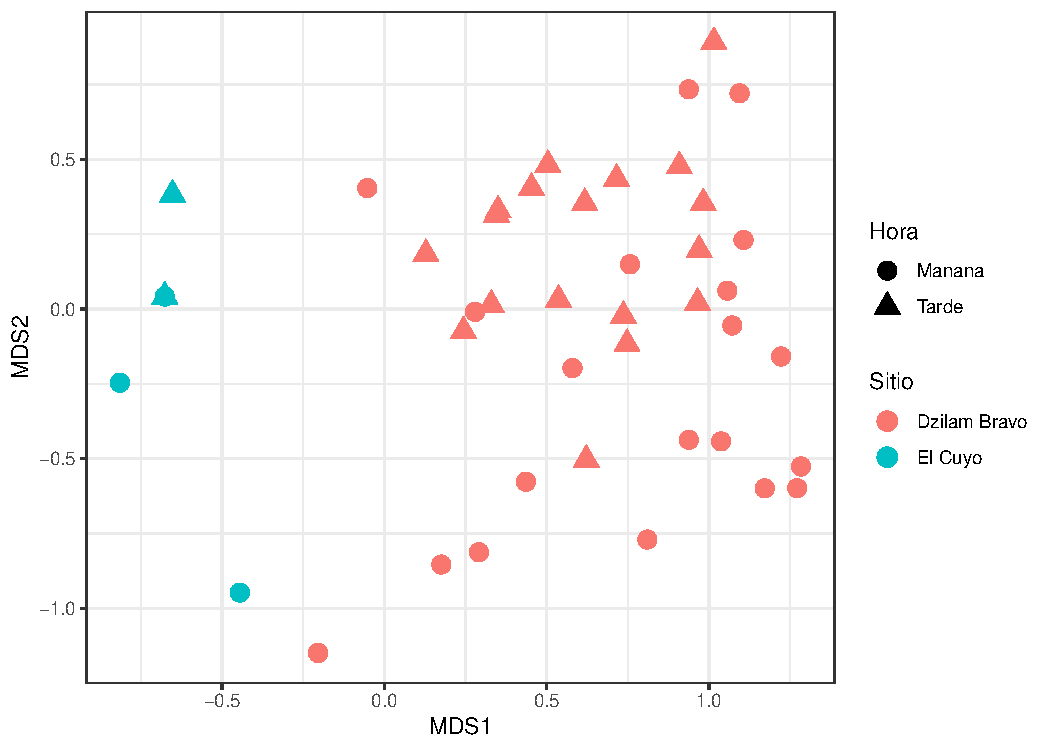
\includegraphics[width=0.5\textwidth,height=\textheight]{Reporte_Campo_files/figure-pdf/fig-mds-1.pdf}

}

\caption{\label{fig-mds}MDS no métrico de las composición y abunndancia
de peces observadas en Dzilam y el Cuyo, en horario matutino y
vespertino.}

\end{figure}

\hypertarget{tables-coming-from-r}{%
\section{Tables coming from R}\label{tables-coming-from-r}}

Tables can also be generated using R chunks, as shown in
Tabla~\ref{tbl-simple} example.

\begin{Shaded}
\begin{Highlighting}[]
\NormalTok{knitr}\SpecialCharTok{::}\FunctionTok{kable}\NormalTok{(}\FunctionTok{head}\NormalTok{(mtcars)[,}\DecValTok{1}\SpecialCharTok{:}\DecValTok{4}\NormalTok{])}
\end{Highlighting}
\end{Shaded}

\hypertarget{tbl-simple}{}
\begin{longtable}[]{@{}lrrrr@{}}
\caption{\label{tbl-simple}Caption centered above table}\tabularnewline
\toprule\noalign{}
& mpg & cyl & disp & hp \\
\midrule\noalign{}
\endfirsthead
\toprule\noalign{}
& mpg & cyl & disp & hp \\
\midrule\noalign{}
\endhead
\bottomrule\noalign{}
\endlastfoot
Mazda RX4 & 21.0 & 6 & 160 & 110 \\
Mazda RX4 Wag & 21.0 & 6 & 160 & 110 \\
Datsun 710 & 22.8 & 4 & 108 & 93 \\
Hornet 4 Drive & 21.4 & 6 & 258 & 110 \\
Hornet Sportabout & 18.7 & 8 & 360 & 175 \\
Valiant & 18.1 & 6 & 225 & 105 \\
\end{longtable}

\hypertarget{discusiuxf3n}{%
\section*{Discusión}\label{discusiuxf3n}}
\addcontentsline{toc}{section}{Discusión}

lang:es

Los resultados muestran una composición de especies distintas en ambos
sitios, esto se ve respaldado gráficamente en la fig.~1, y numéricamente
con el valor obtenido de PERMANOVA {[}poner el valor{]}, proponemos que
una de las causas principales de este cambio se puede deber a las
condiciones ambientales, tanto de la columna de agua como de el
sustrato, se puede ver además en la fig.~1 que también se ve un patrón
entre las especies observadas en la mañana y la tarde en ambos sitios.

\hypertarget{conclusiuxf3n}{%
\section*{Conclusión}\label{conclusiuxf3n}}
\addcontentsline{toc}{section}{Conclusión}

El protocolo AGRRA para peces brinda una opción de muestreo
estandarizado y accesible no solo para fines de docencia si no para la
investigación formal, los resultados

\hypertarget{reconocimiento}{%
\subsection{Reconocimiento}\label{reconocimiento}}

Esta investigación va dedicada al Dr.~Edlin Guerra y la Dra. Maria
Muciño por guiarnos en la realización de la misma. Tambien a don Chuy
por invitarnos unas aguas de coco, una disculpa a este último porque no
nos la acabamos y tuvimos que tirar dos porque ya olían gacho, para
proximos estudios sugerimos dar nuestra tanda. Abrazo, abrazo, beso,
beso, abrazo, abrazo, besote, abracito, beso, besito.


\renewcommand\refname{References}
  \bibliography{bibliography.bib}


\end{document}
